\shorthandoff{"}
\chapter{Forschungsergebnisse}
\label{ch:ergebnisse}

\section{Fähigkeiten und Präferenzen der Mitarbeiter}
\label{ch:ergebnisse:analyse}
An der Umfrage unter den Projektmitarbeitern haben N=23 Personen aus dem Fachbereich \acl{JES} der EXXETA AG teilgenommen. Diese Angestellten haben insgesamt 643 Kompetenzbewertungen im Intranet des Unternehmens abgegeben, was ca. 28 vergebenen Beurteilungen pro Person entspricht. Die Bewertungen verteilen sich auf insgesamt 212 der \anzFaehigkeiten unterschiedlichen im Intranet gespeicherten Fähigkeiten. Java ist mit 16 Beurteilungen die meist bewertete Kompetenz.

Abbildung \ref{fig:ergebnisse:analyse:abb1} zeigt die bewerteten Fähigkeiten sortiert nach Anzahl an Beurteilungen. Dabei ist der in Kapitel \ref{ch:empfehlungssysteme:cf:speicherbasiert} vorgestellte lange (Ratten-)Schwanz gut erkennbar. Dieser ist jedoch weniger stark ausgeprägt, als in der Referenzdarstellung aus Abbildung \ref{fig:empfehlungssysteme:cf:speicherbasiert:abb1}.

\begin{figure}[h]
	\centering
	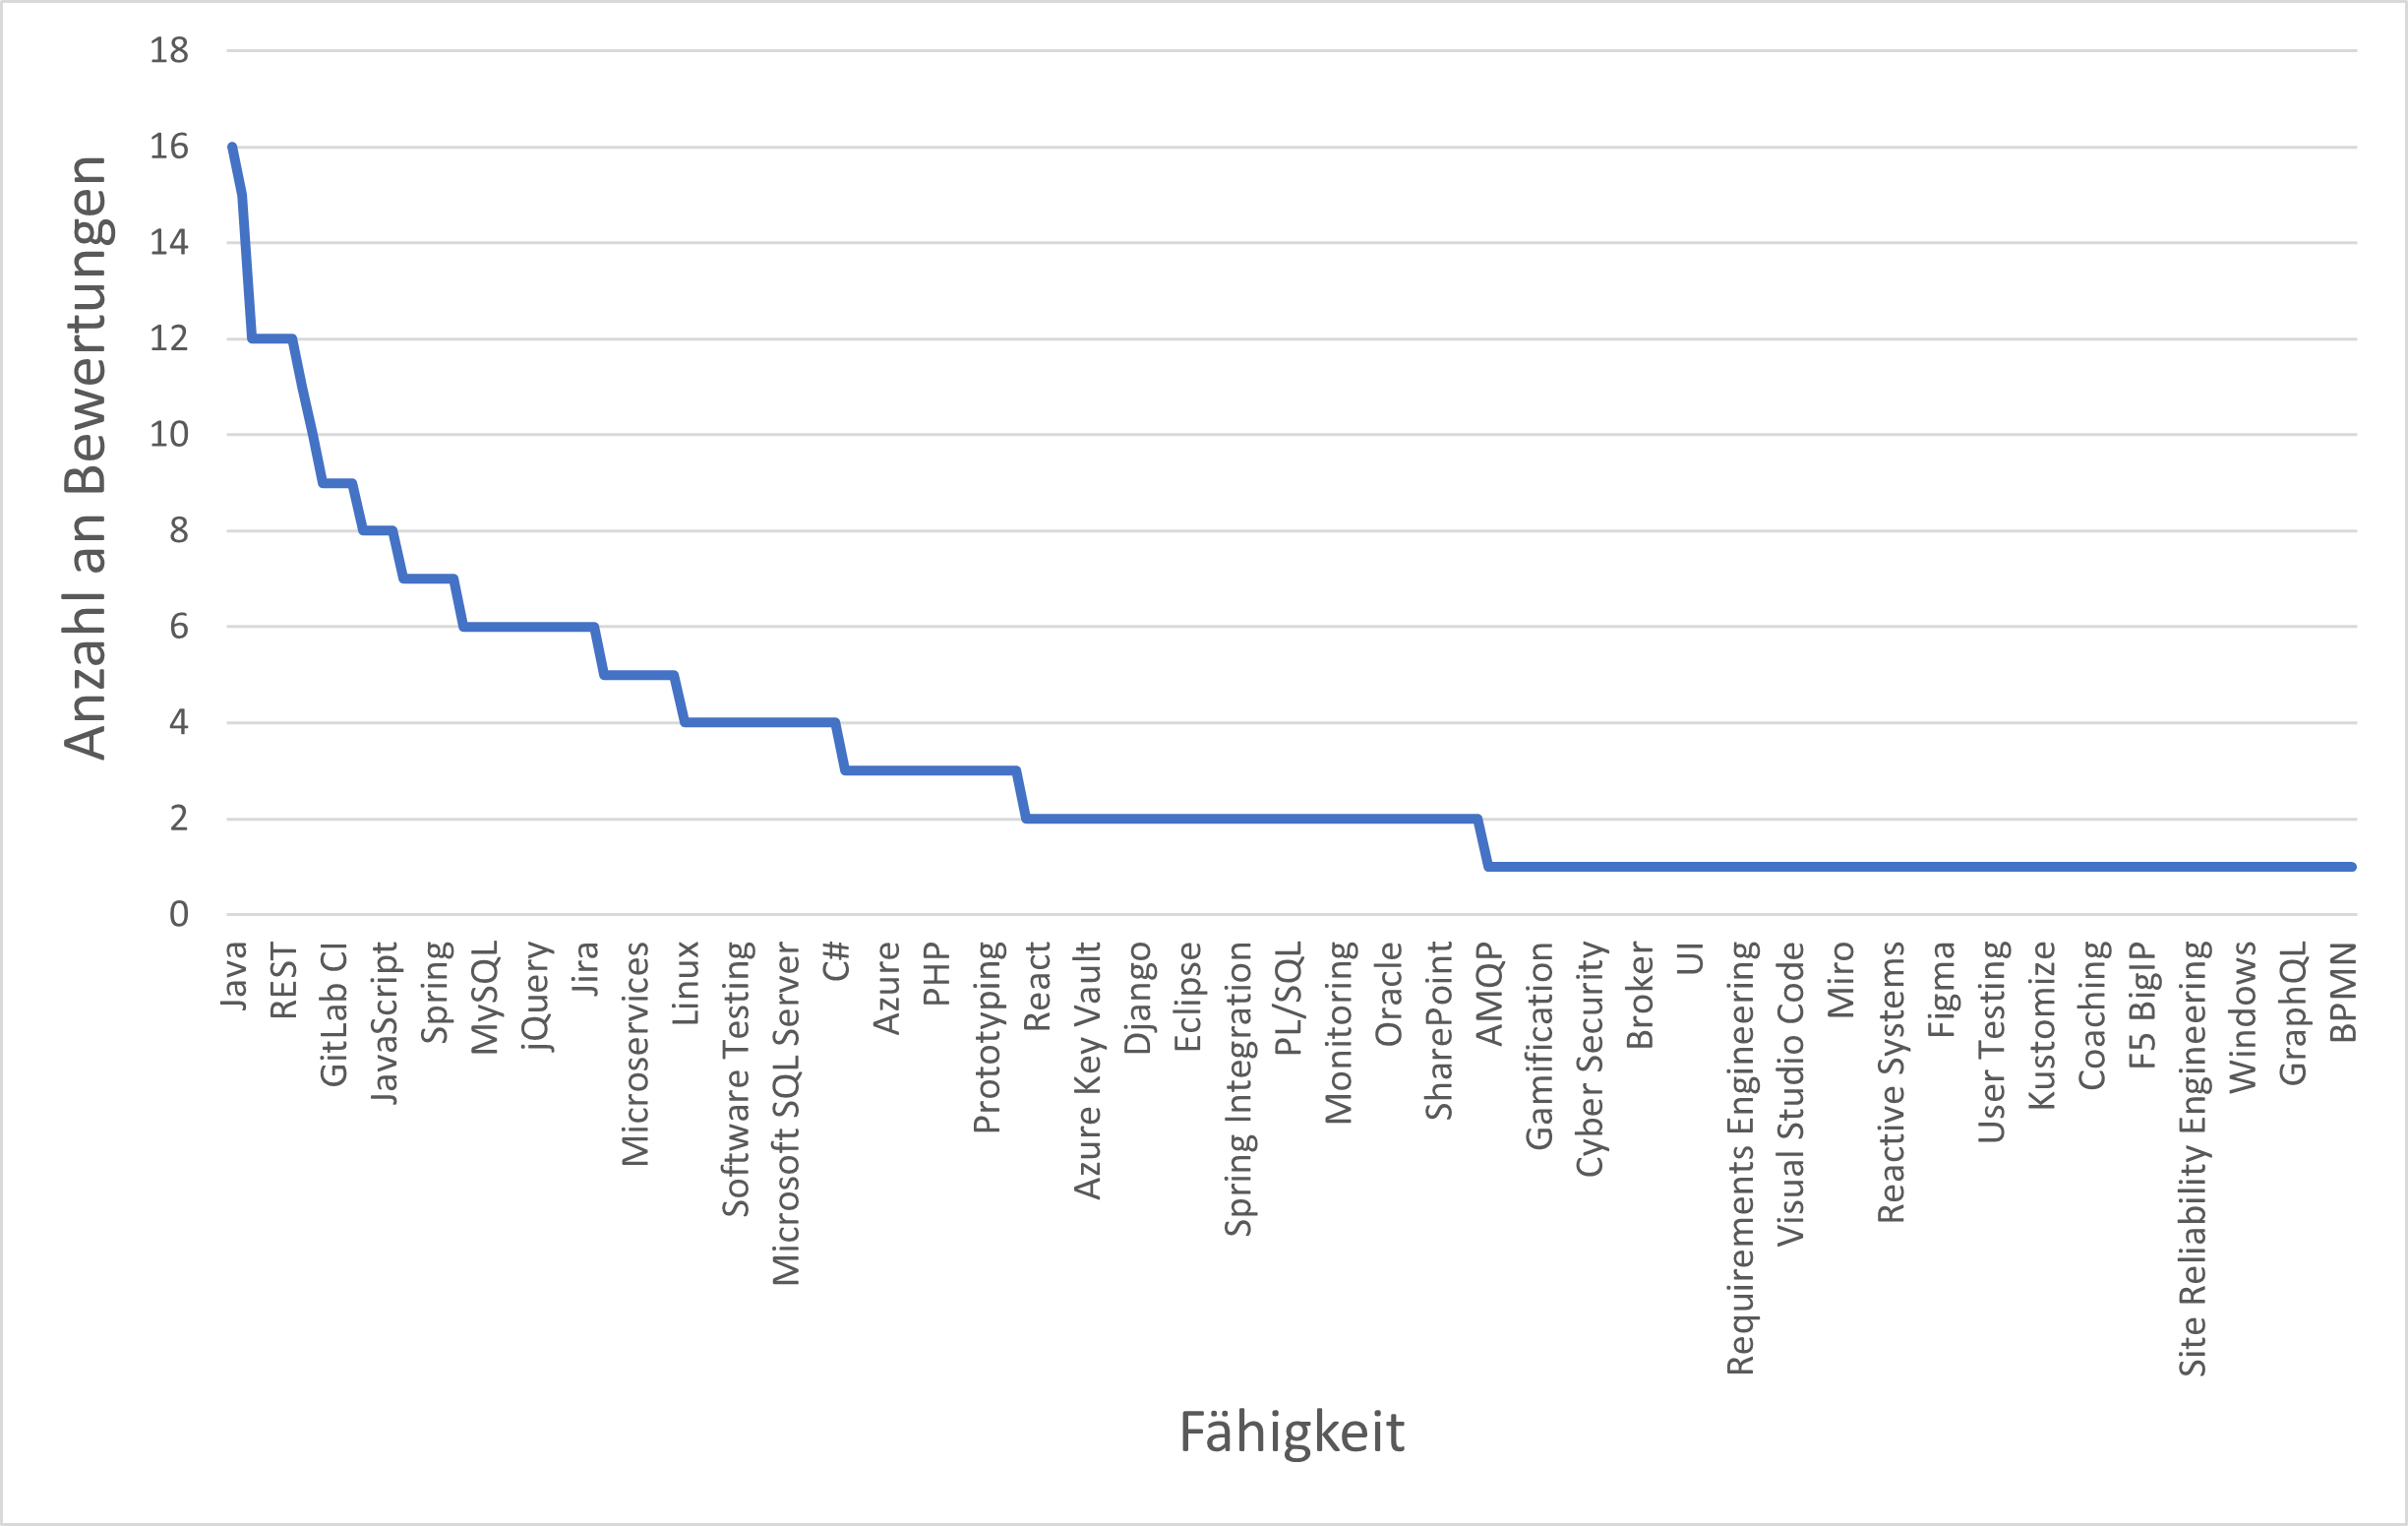
\includegraphics[width=1\textwidth]{gfx/long-tail-intranet.png}
	\caption{Langer (Ratten-)Schwanz bei den Fähigkeitsbewertungen im EXXETA-Intranet}
	\label{fig:ergebnisse:analyse:abb1}
\end{figure}

In Abbildung \ref{fig:ergebnisse:analyse:abb1} ist bezüglich des langen (Ratten-)Schwanzes festzustellen, dass neun bzw. etwa 4.3 Prozent aller Fähigkeiten über zehn oder mehr Bewertungen verfügen. Dagegen haben 151 bzw. etwa 71.2 Prozent aller Kompetenzen drei oder weniger Beurteilungen.

In den vorliegenden Daten des Intranets ist darüber hinaus zu beobachten, dass vier bzw. etwa 17.4 Prozent der Mitarbeiter keine einzige Fähigkeit bewertet haben. Der Grund hierfür ist, dass diese Angestellten seit Einführung des Kompetenz-Bewertungssystems durchgehend in einem Projekt tätig sind und daher von ihrer Führungskraft noch nicht zur Pflege ihrer Fähigkeiten aufgefordert wurden.

Bei der Umfrage zu den Präferenzen haben die Mitarbeiter insgesamt 1408 Bewertungen abgegeben, welche sich auf 370 einzelne Kompetenzen verteilen. Dies entspricht knapp über 61 abgegebenen Wünschen pro Mitarbeiter. Git ist mit 18 Beurteilungen die meist bewertete Fähigkeit. Wie in Abbildung \ref{fig:ergebnisse:analyse:abb2} zu erkennen, deutet sich auch hinsichtlich der Präferenzen der Angestellten ein langer (Ratten-)Schwanz an, wenn die Fähigkeiten nach Anzahl an Beurteilungen sortiert dargestellt werden.
 
\begin{figure}[h]
	\centering
	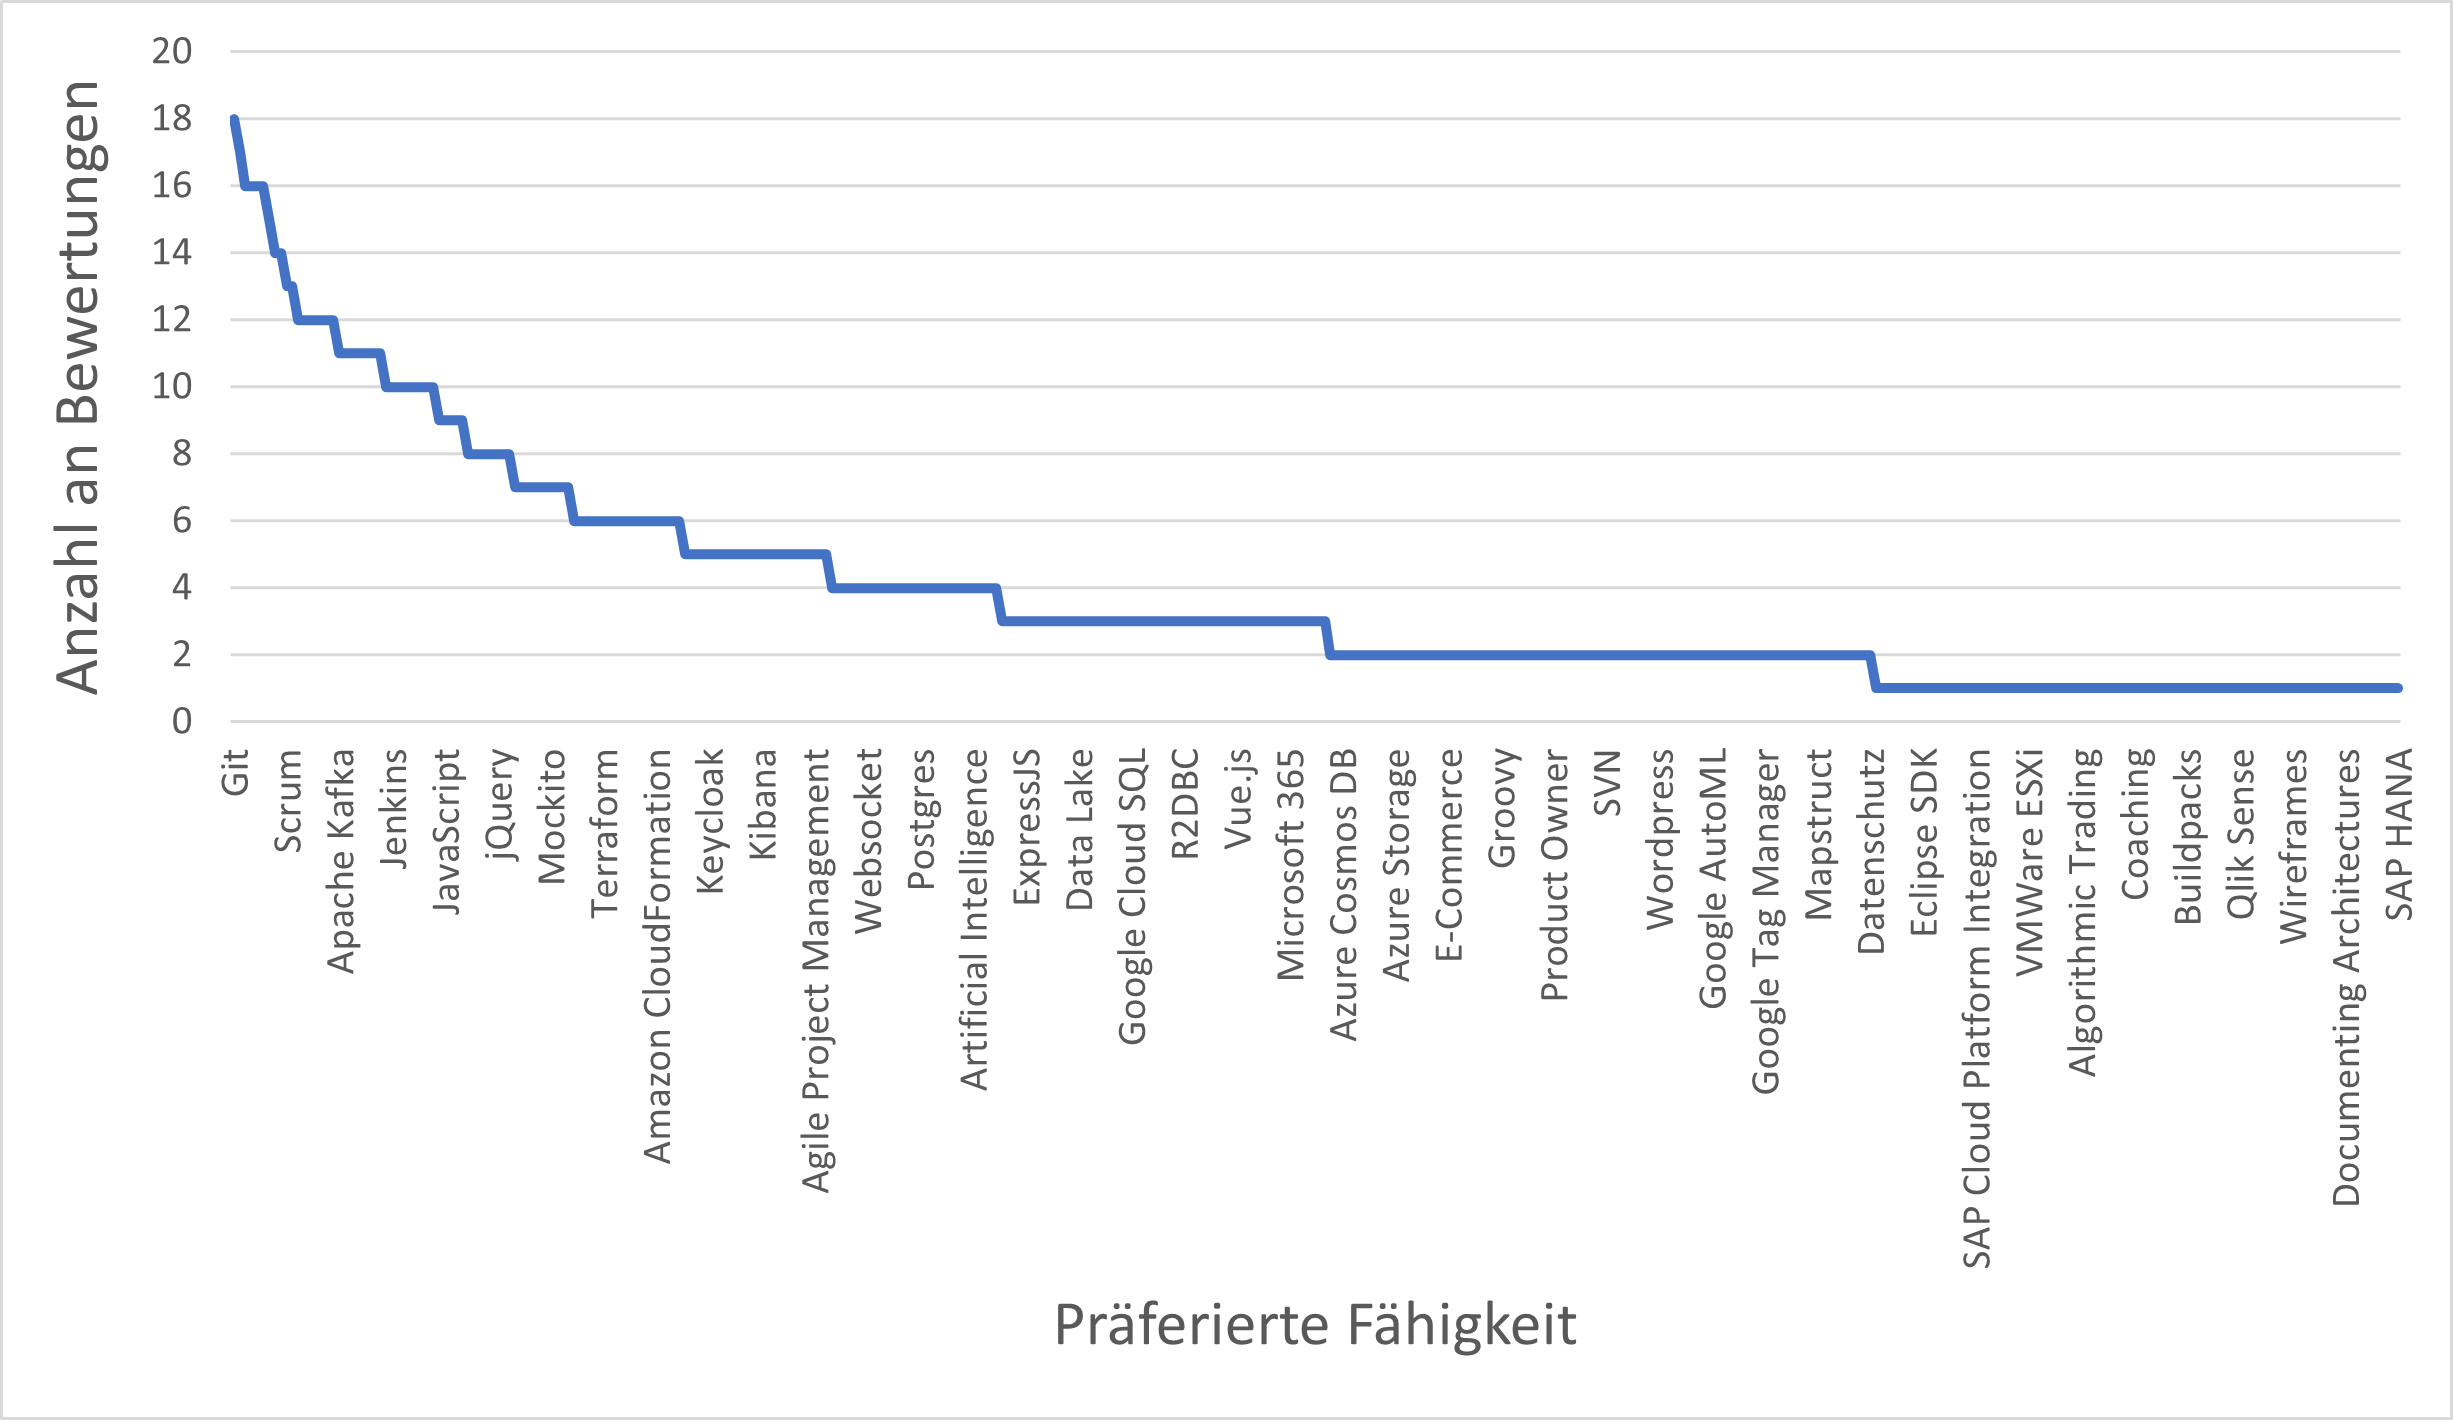
\includegraphics[width=1\textwidth]{gfx/long-tail-praeferenzen.png}
	\caption{Langer (Ratten-)Schwanz bei den präferierten Fähigkeiten der Mitarbeiter}
	\label{fig:ergebnisse:analyse:abb2}
\end{figure}

Zu Abbildung \ref{fig:ergebnisse:analyse:abb2} ist festzustellen, dass 18 bzw. etwa 4.9 Prozent aller Fähigkeiten von zwölf oder mehr Mitarbeitern präferiert werden. Dem gegenüber stehen 268 bzw. etwa 72.4 Prozent aller Kompetenzen, welche vier oder weniger Angestellte als Wunsch angaben. Bei der Umfrage gab es keinen Mitarbeiter, welcher keine einzige Fähigkeit als Präferenz ausgewählte.

Bei der gemeinsamen Betrachtung von Kompetenzen und Wünschen ist auf Mitarbeiterebene festzustellen, dass ein durchschnittlicher Angestellter ca. 74.7 Fähigkeiten bewertet hat. Wie in Abbildung \ref{fig:ergebnisse:analyse:abb3} zu erkennen, beherrscht dieser bereits etwa 28 bzw. ca. 37.4 Prozent der beurteilten Kompetenzen. Von diesen vorhandenen Fähigkeiten präferiert er jedoch nur ca. 14.5 Kompetenzen, also knapp über die Hälfte. Demgegenüber stehen ca. 46.7 bzw. etwa 62.6 Prozent Fähigkeiten, welche der Angestellte zwar präferiert, aber noch nicht beherrscht.

\begin{figure}[h]
	\centering
	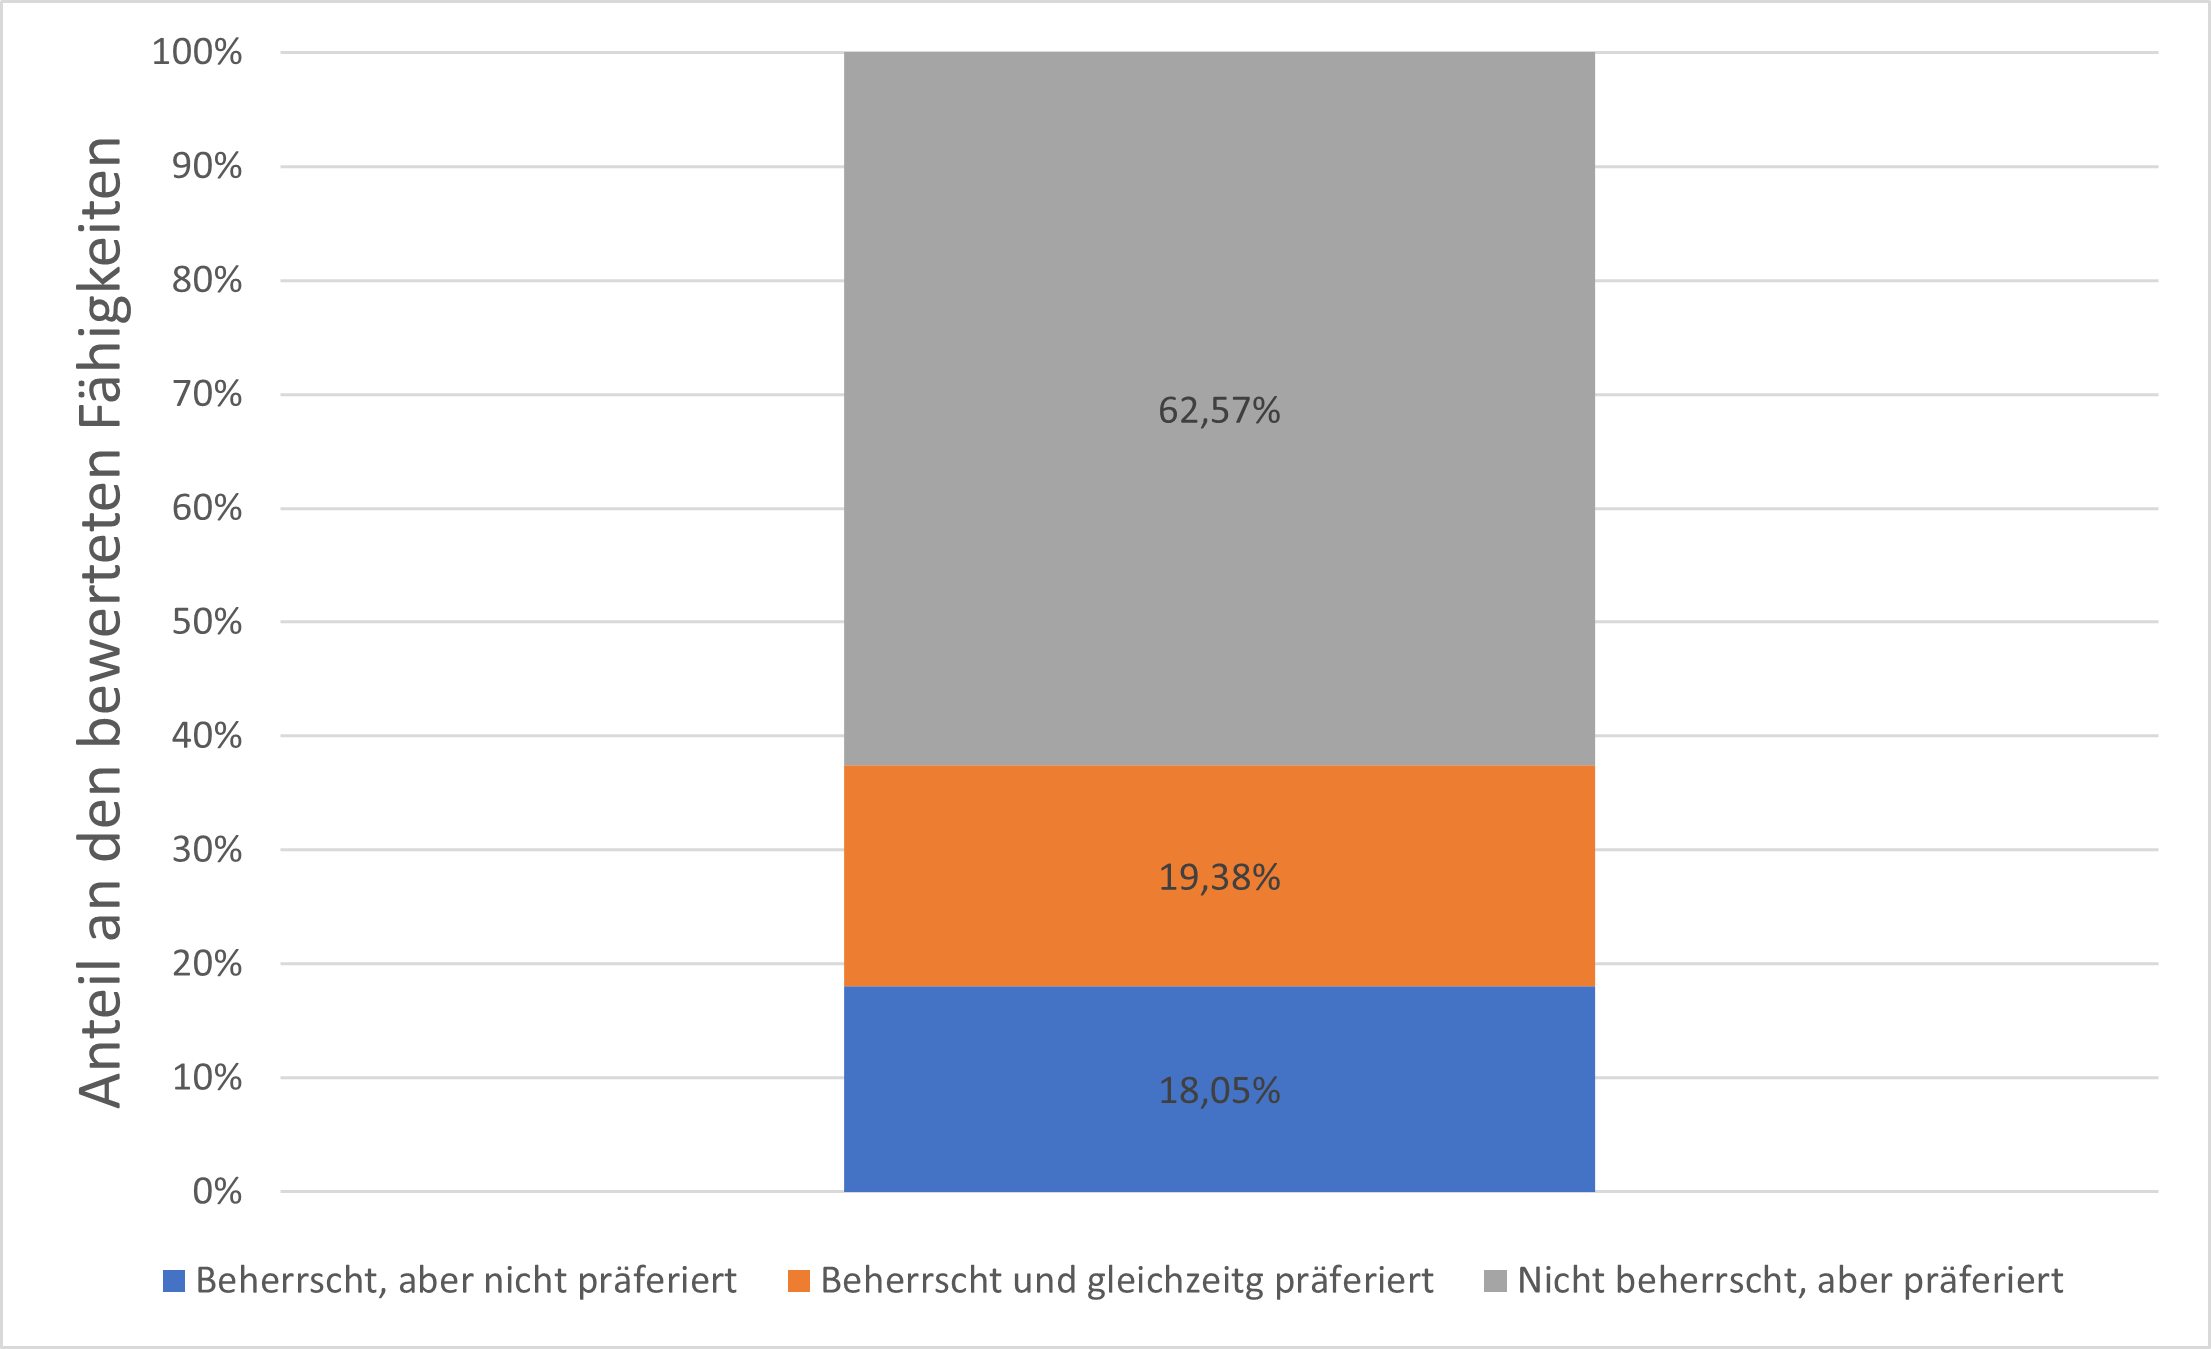
\includegraphics[width=1\textwidth]{gfx/auswertung-anteil-an-faehigkeiten.png}
	\caption{Anteil beherrschter und präferierter Fähigkeiten bei einem durchschnittlichen Mitarbeiter}
	\label{fig:ergebnisse:analyse:abb3}
\end{figure}


\newpage
Bei der gemeinsamen Betrachtung von beherrschten und präferierten Fähigkeiten ist festzustellen, dass die Mitarbeiter 192 ihrer 212 beherrschten Kompetenzen, also über 90 Prozent, ebenfalls präferieren. Gleichzeitig bedeutet dies, dass die Angestellten 178 bzw. über 48 Prozent aller Kompetenzen noch nicht beherrschen, welche diese präferieren. Hierzu ist festzustellen, dass die Mitarbeiter häufig Fähigkeiten als Wunsch angeben, 

- Wie viele Cloud, KI? --> Wie viele nur 1 Bewertung (Ausreißer)


- Kein Coldstart bei Präferenzen
- Es sind immer mind. 19 andere Personen auf einem Skill verbunden

Projekt A: unilateral/bilateral\\
Projekt B: bilateral/unilateral\\
Projekt C: bilateral/unilateral\\
Projekt D: unilateral/bilateral\\
Projekt E: unilateral/bilateral

\shorthandon{"}
